\section{產品服務與內容}

\subsection{產品與服務內容}

ProgLearn程式教學系統,以程式教師為中心設計,強調師生間的即時互動,提供0延遲直播、課程與作業管理,以及具有即時反饋功能的數位儀表板、講義視覺化編輯、智慧引導和自動批改等多功能(圖\ref{fig:Classroom})。

\begin{figure}[H]
  \begin{subfigure}{0.5\linewidth}
    \centering
    %   \href{https://raw.githubusercontent.com/programingtw/proglearn-plan/main/img/student.png}{ 
    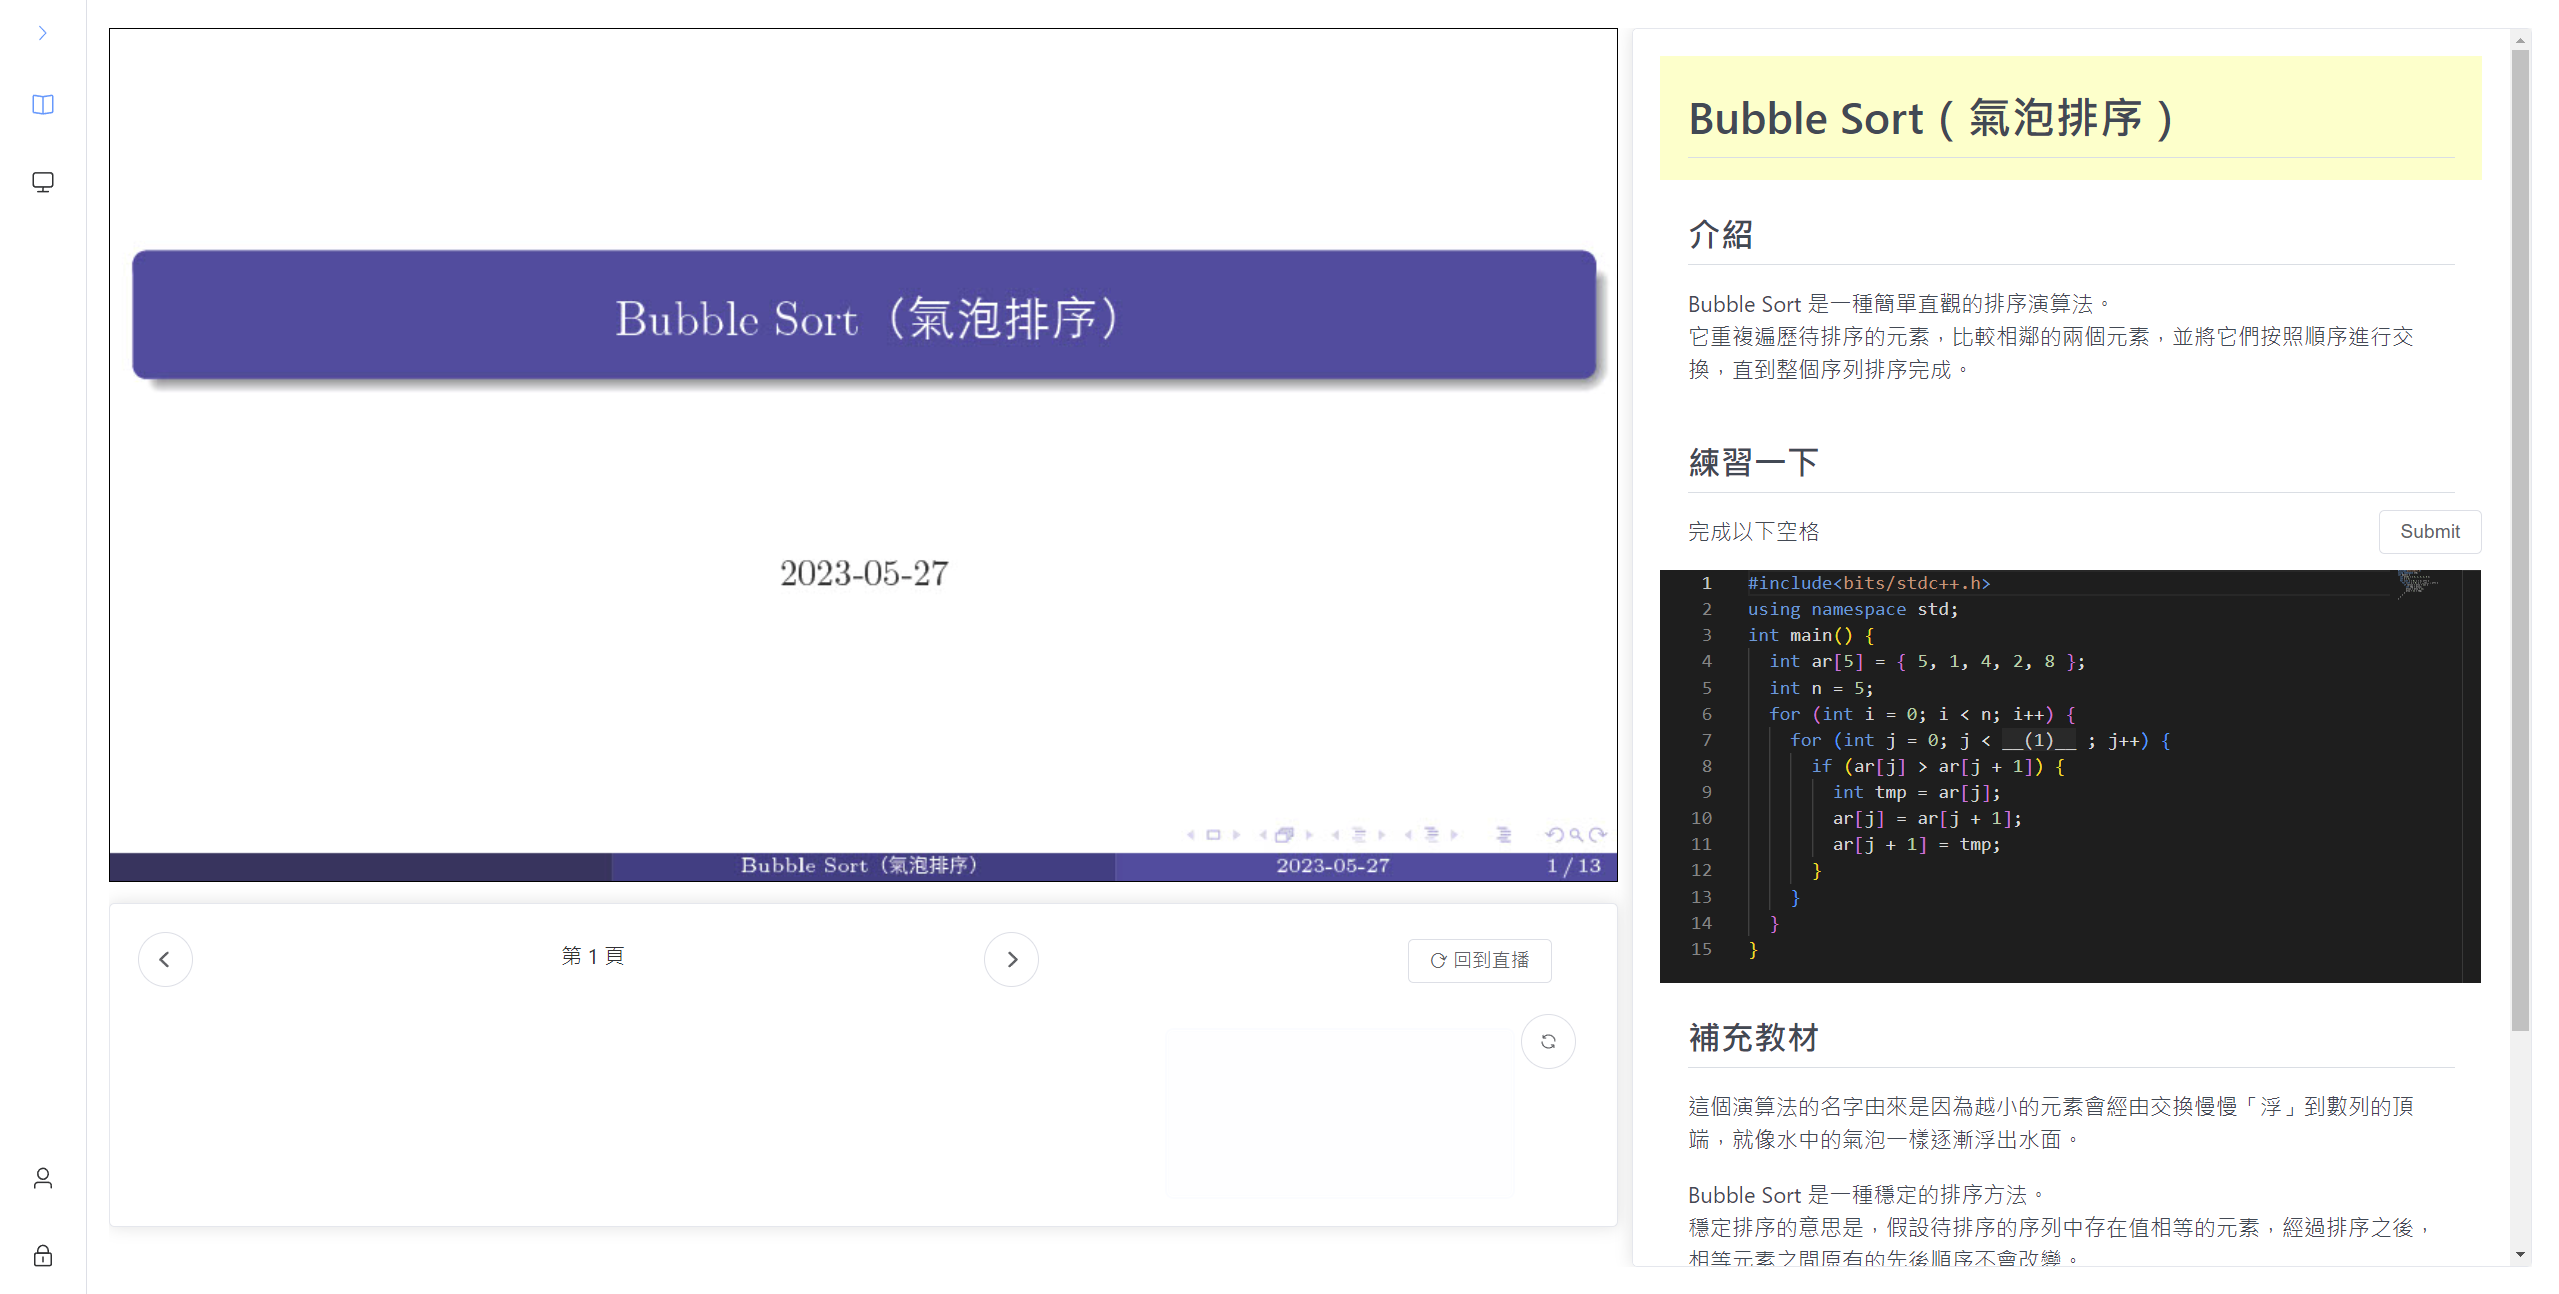
\includegraphics[width=1\textwidth]{images/student.png}
    %   }
    \caption{學生課堂頁面}
  \end{subfigure}
  \begin{subfigure}{0.5\linewidth}
    \centering
        % \href{https://raw.githubusercontent.com/programingtw/proglearn-plan/main/img/teacher.png}{ 
    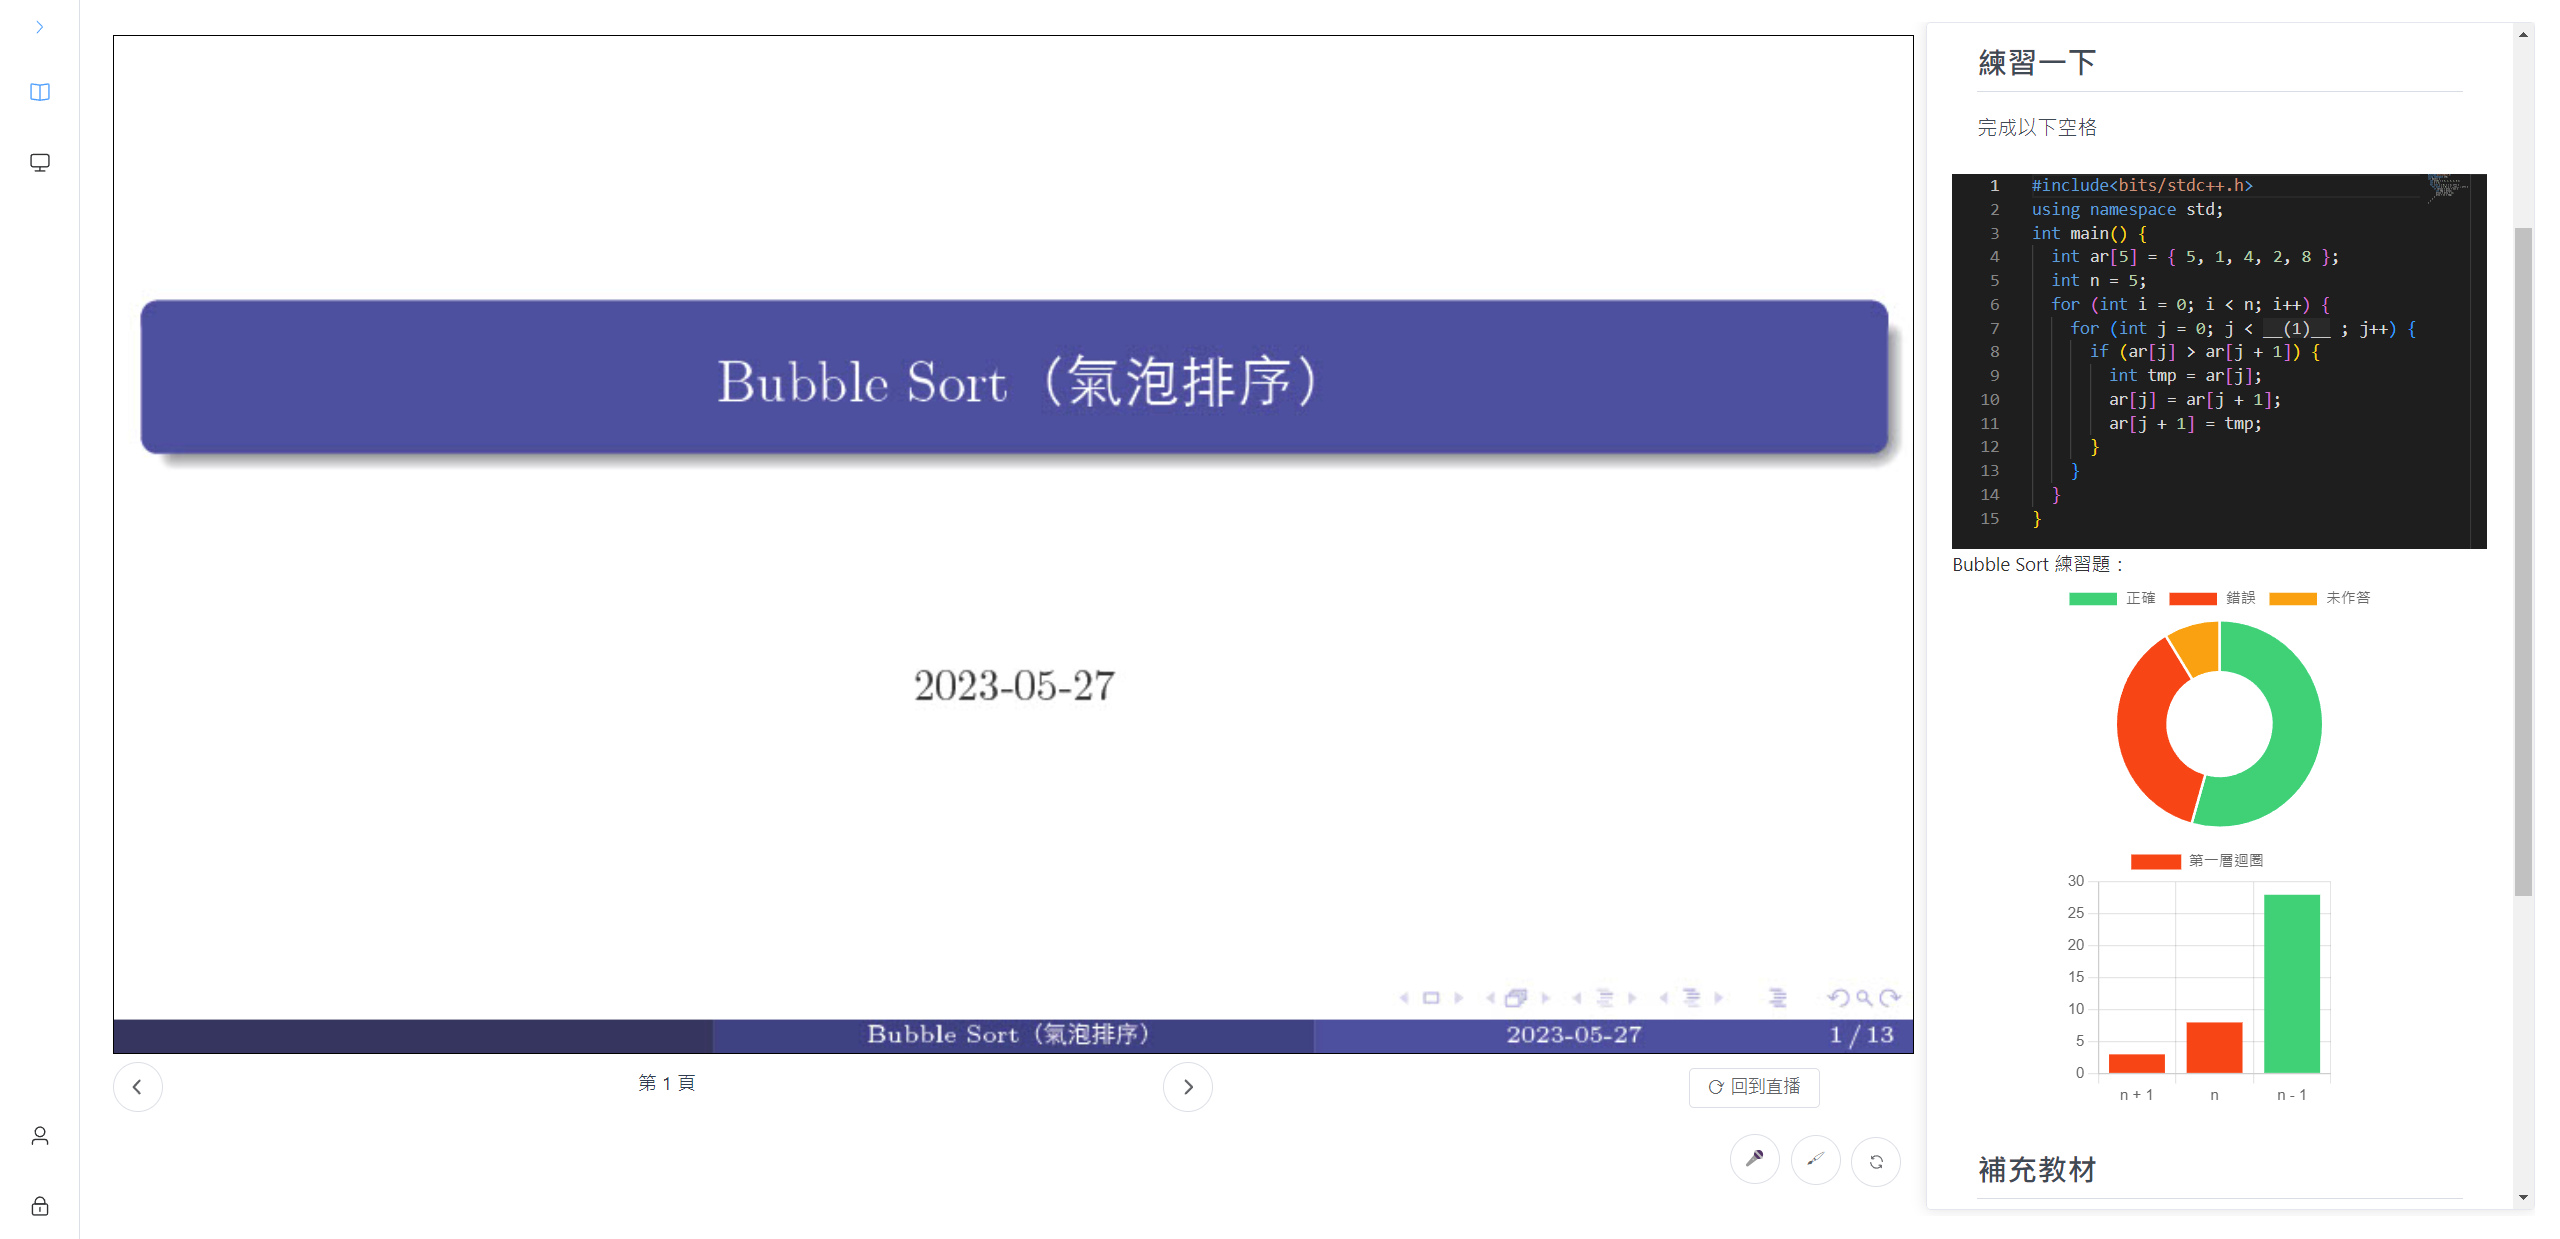
\includegraphics[width=1\textwidth]{images/teacher.png}
        % }
    \caption{教師課堂頁面}
  \end{subfigure}
  \caption{課堂介面}
  \label{fig:Classroom}
\end{figure}

\subsubsection{直播功能}

\begin{figure}[H]
  \centering
  %   \href{https://raw.githubusercontent.com/programingtw/proglearn-plan/main/img/live.png}{ 
  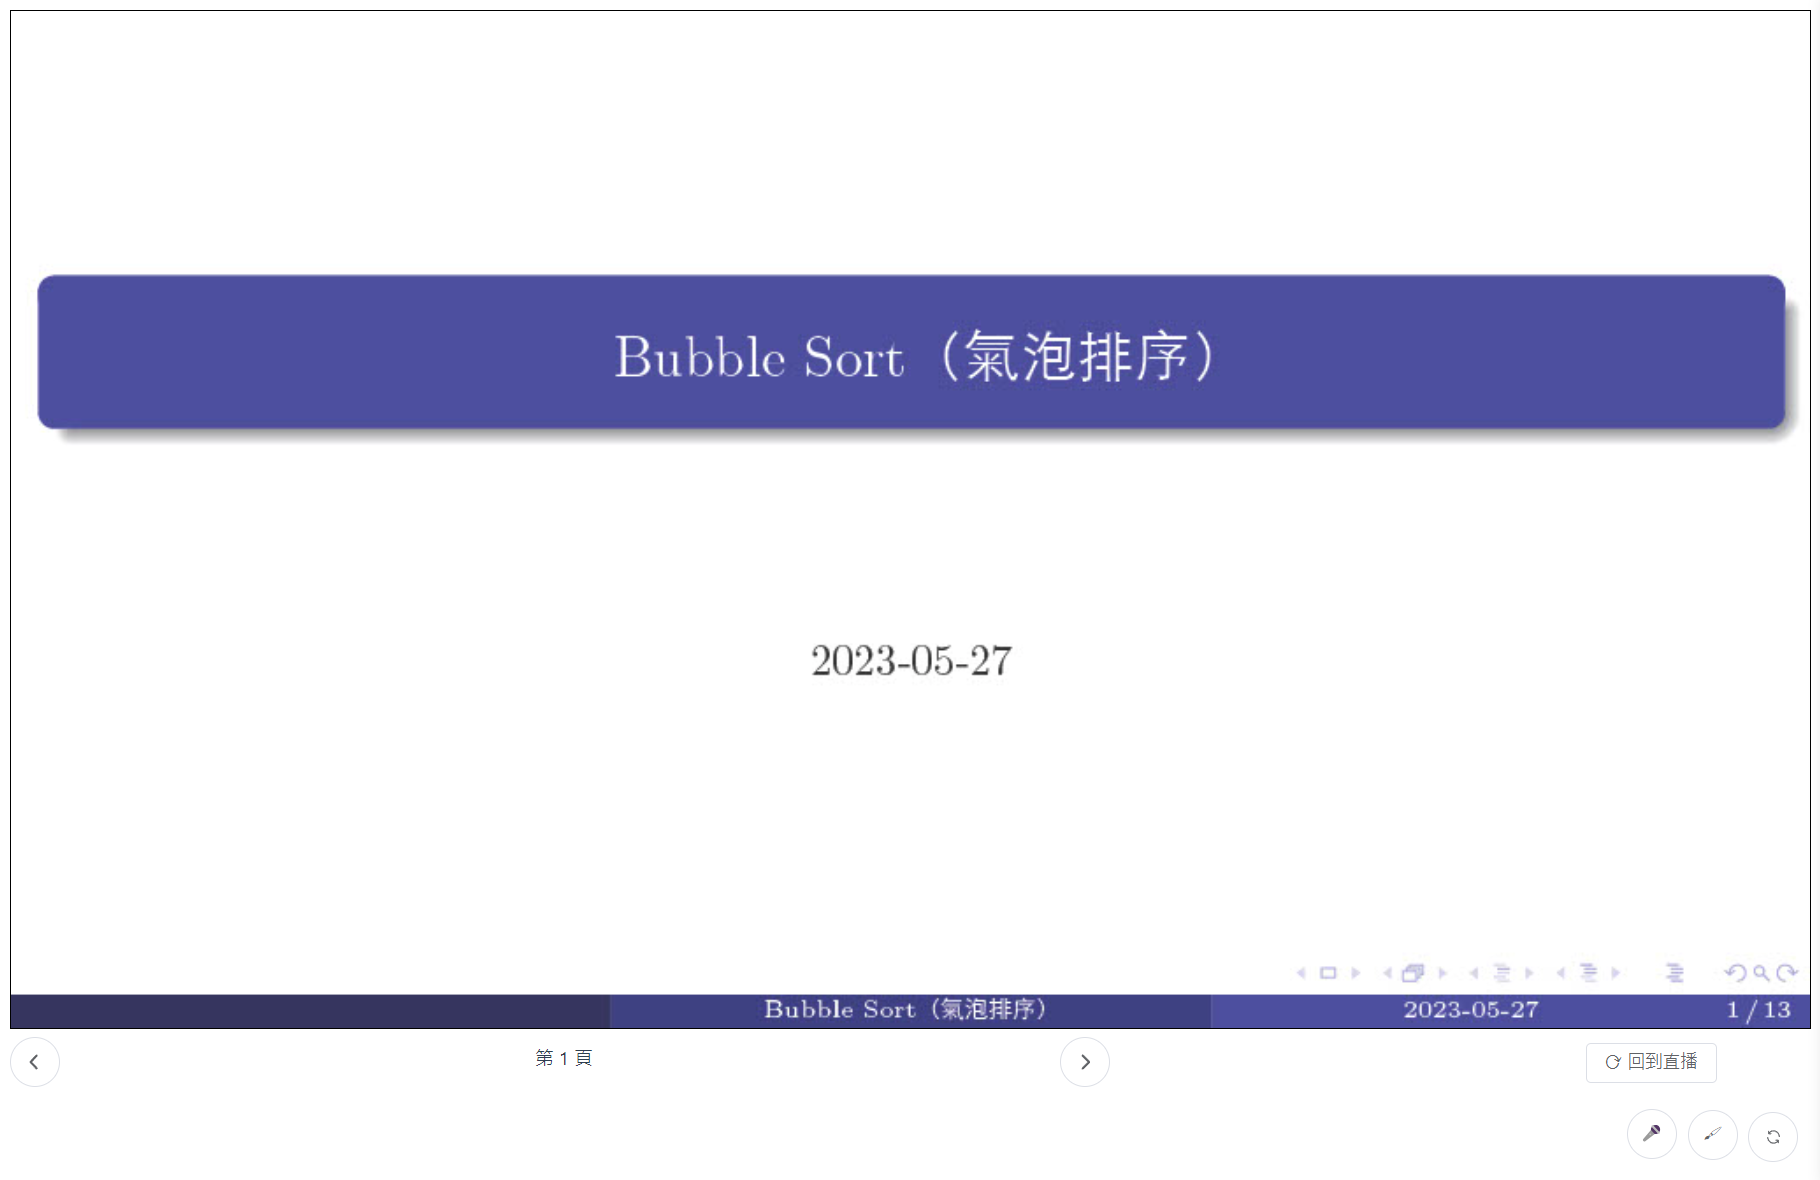
\includegraphics[width=0.5\textwidth]{images/streaming.png}
  %   }
  \caption{直播功能區}
\end{figure}

直播功能區位在課堂介面的左半部。此直播功能不同於往常的影像傳輸,而是記錄教師在投影片上的所有操作。包含換頁、繪畫、游標軌跡和聲音實時同步到學生端的介面上,然後存儲在直播記錄中,方便回顧與學習。
因此相比於Zoom、Meet等視訊會議工具,具有更低的網路延遲與頻寬需求,並且更加穩定。

在實體教學中可以作為教學的輔助工具。在線上與偏鄉教學中,其更低的硬體需求,可以作為主要的教學工具。

\subsubsection{互動式講義}

\begin{figure}[H]
  \begin{subfigure}{0.5\linewidth}
    \centering
    %   \href{https://raw.githubusercontent.com/programingtw/proglearn-plan/main/img/student.png}{ 
    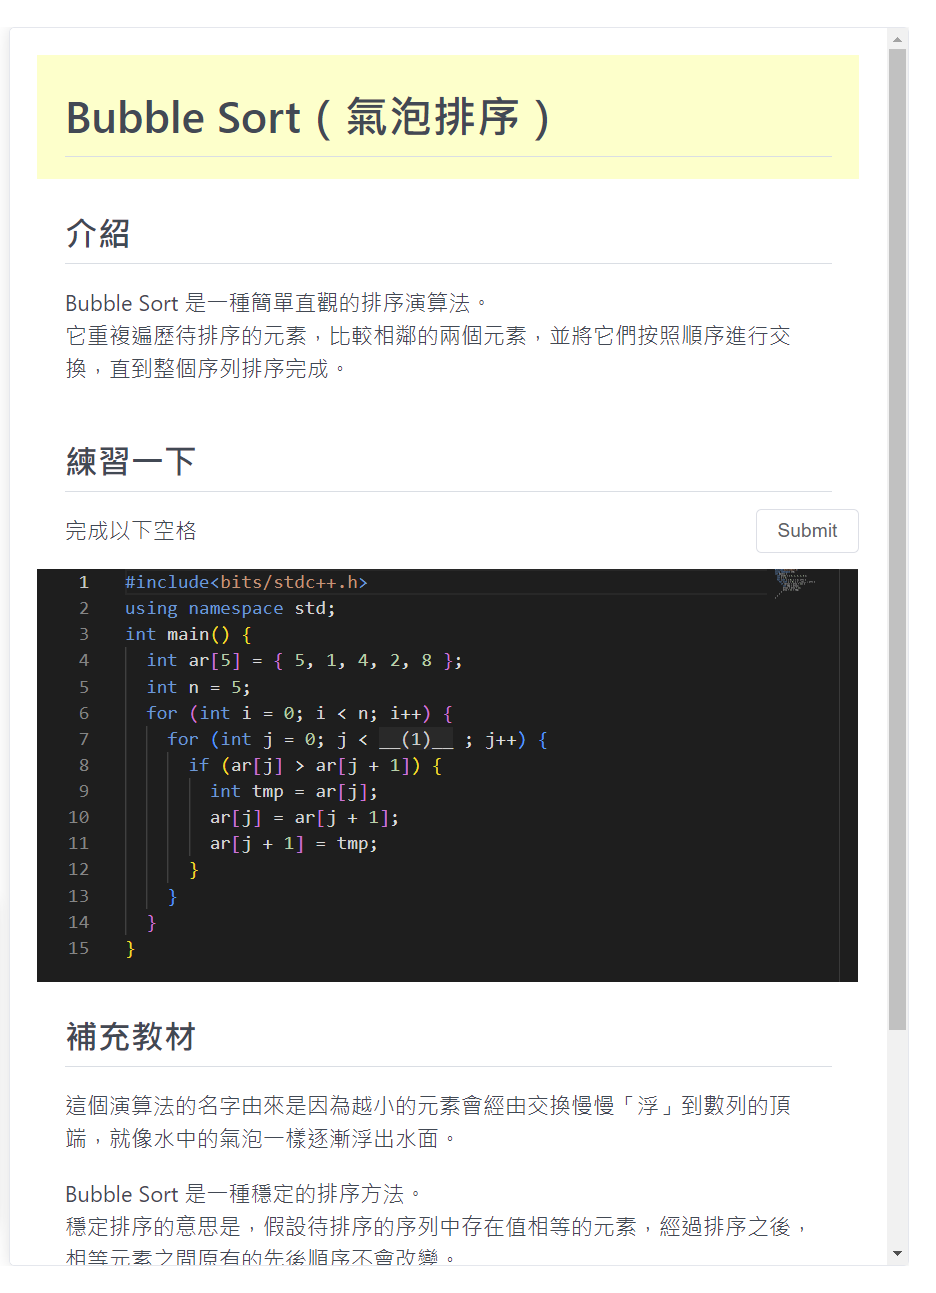
\includegraphics[width=0.5\textwidth]{images/side-s.png}
    %   }
    \caption{學生課堂頁面}
    \label{fig:student}
  \end{subfigure}
  \begin{subfigure}{0.5\linewidth}
    \centering
        % \href{https://raw.githubusercontent.com/programingtw/proglearn-plan/main/img/teacher.png}{ 
    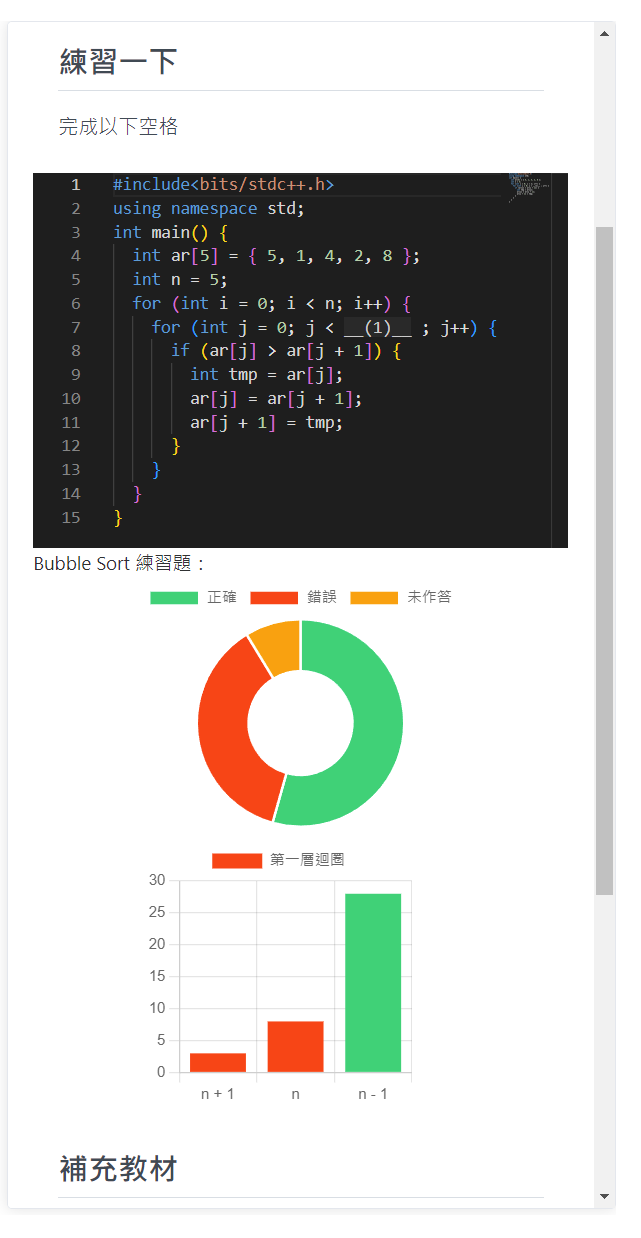
\includegraphics[width=0.5\textwidth]{images/side-t.png}
        % }
    \caption{教師課堂頁面}
    \label{fig:teacher}
  \end{subfigure}
  \caption{互動式講義區塊}
\end{figure}

互動式講義位在課堂介面的右半部。目的是在課堂中能提供師生間互動的橋樑,並作為教學與學習的輔助工具。其相關功能可細分為以下四點:

\begin{enumerate}
  \setlength{\parindent}{2em}

  \item 智慧引導
  \par 透過淺黃色區塊,向學生指引出當前直播對應到講義上的哪些部分(圖\ref{fig:student})。
  
  \item 即時反饋(數位儀表板)
  \par 為教師提供學生的課堂作答情況,即時了解學生的學習狀況(圖\ref{fig:teacher})。

  \item 自動批改
  \par 為學生提供課堂上的程式作答功能,透過AI即時批改課堂習題。其技術也應用於作業管理中(圖\ref{fig:problem})。
  
  \begin{figure}[H]
    \begin{subfigure}{0.5\linewidth}
      \centering
      % \href{https://raw.githubusercontent.com/programingtw/proglearn-plan/main/2023全國大專校院智慧創新暨跨域整合創作競賽/img/problem.png}{
        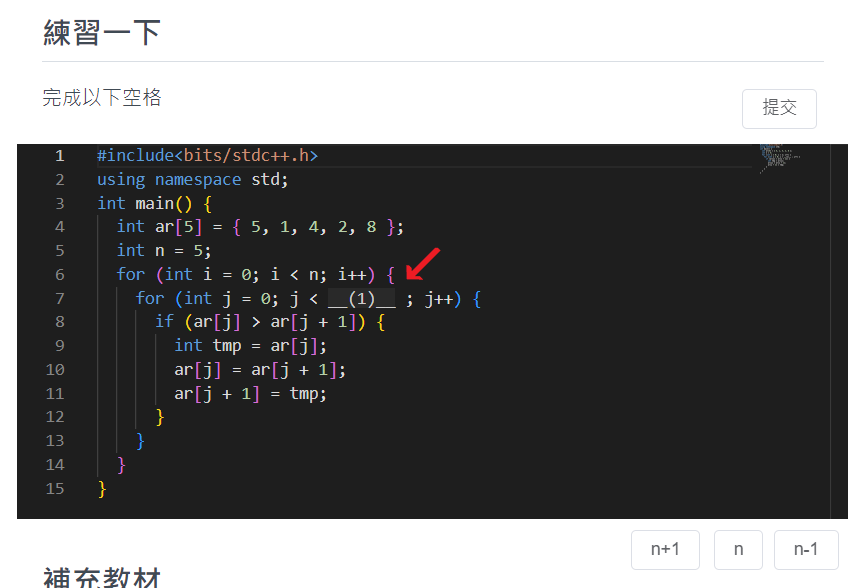
\includegraphics[width=1\textwidth]{images/problem.png}
      % }
      \caption{作答前}
    \end{subfigure}
    \begin{subfigure}{0.5\linewidth}
      \centering
      % \href{https://raw.githubusercontent.com/programingtw/proglearn-plan/main/2023全國大專校院智慧創新暨跨域整合創作競賽/img/problem2.png}{
        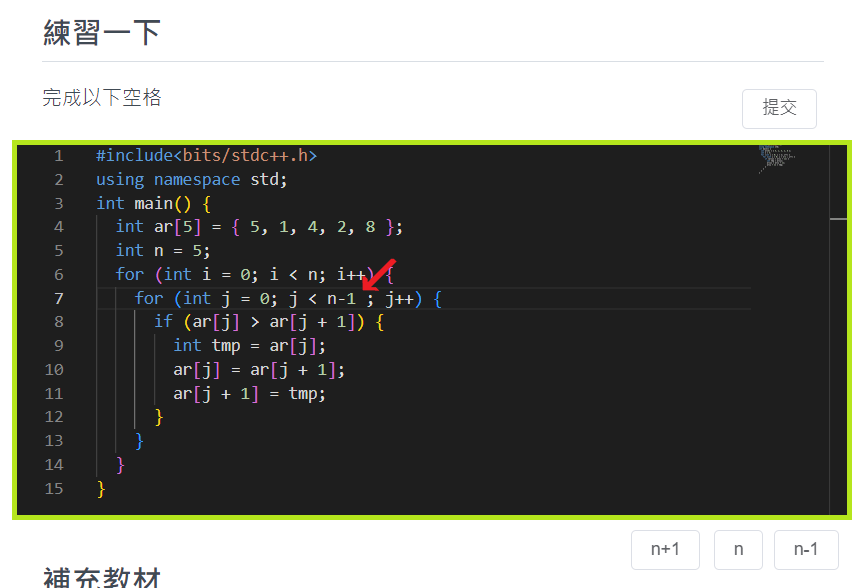
\includegraphics[width=1\textwidth]{images/problem-ac.png}
      % }
      \caption{作答後}
    \end{subfigure}
    \caption[互動式講義的程式題]{互動式講義的程式題:點擊下方選項後,會自動將選項插入到程式碼中(紅色箭頭處)。提交後會以不同的顏色框線即時顯示結果,綠色為作答正確,紅色為作答錯誤。}
    \label{fig:problem}
  \end{figure}

  \item 講義視覺化編輯
  \par 為教師提供編輯講義的功能。為實現投影片和講義內容的智慧引導,我們參考了影片剪輯軟體的設計思路,採用了時間軸的概念。將講義分成不同類型的小區塊,並在時間軸上將這些區塊組合成完整的講義內容(圖\ref{fig:edit})。
  \par 在編排講義時,教師可以輕鬆地將這些區塊拖曳到時間軸中。腳本區的時間軸對應著投影片的頁數,因此講義的不同區塊能夠與投影片緊密連接(圖\ref{fig:time})。在課堂中,當老師切換到特定的頁數時,就能自動在講義中引導學生目前的上課內容。

  \begin{figure}[H]
    \begin{subfigure}{0.5\linewidth}
      \centering
      %   \href{https://raw.githubusercontent.com/programingtw/proglearn-plan/main/img/list.png}{ 
      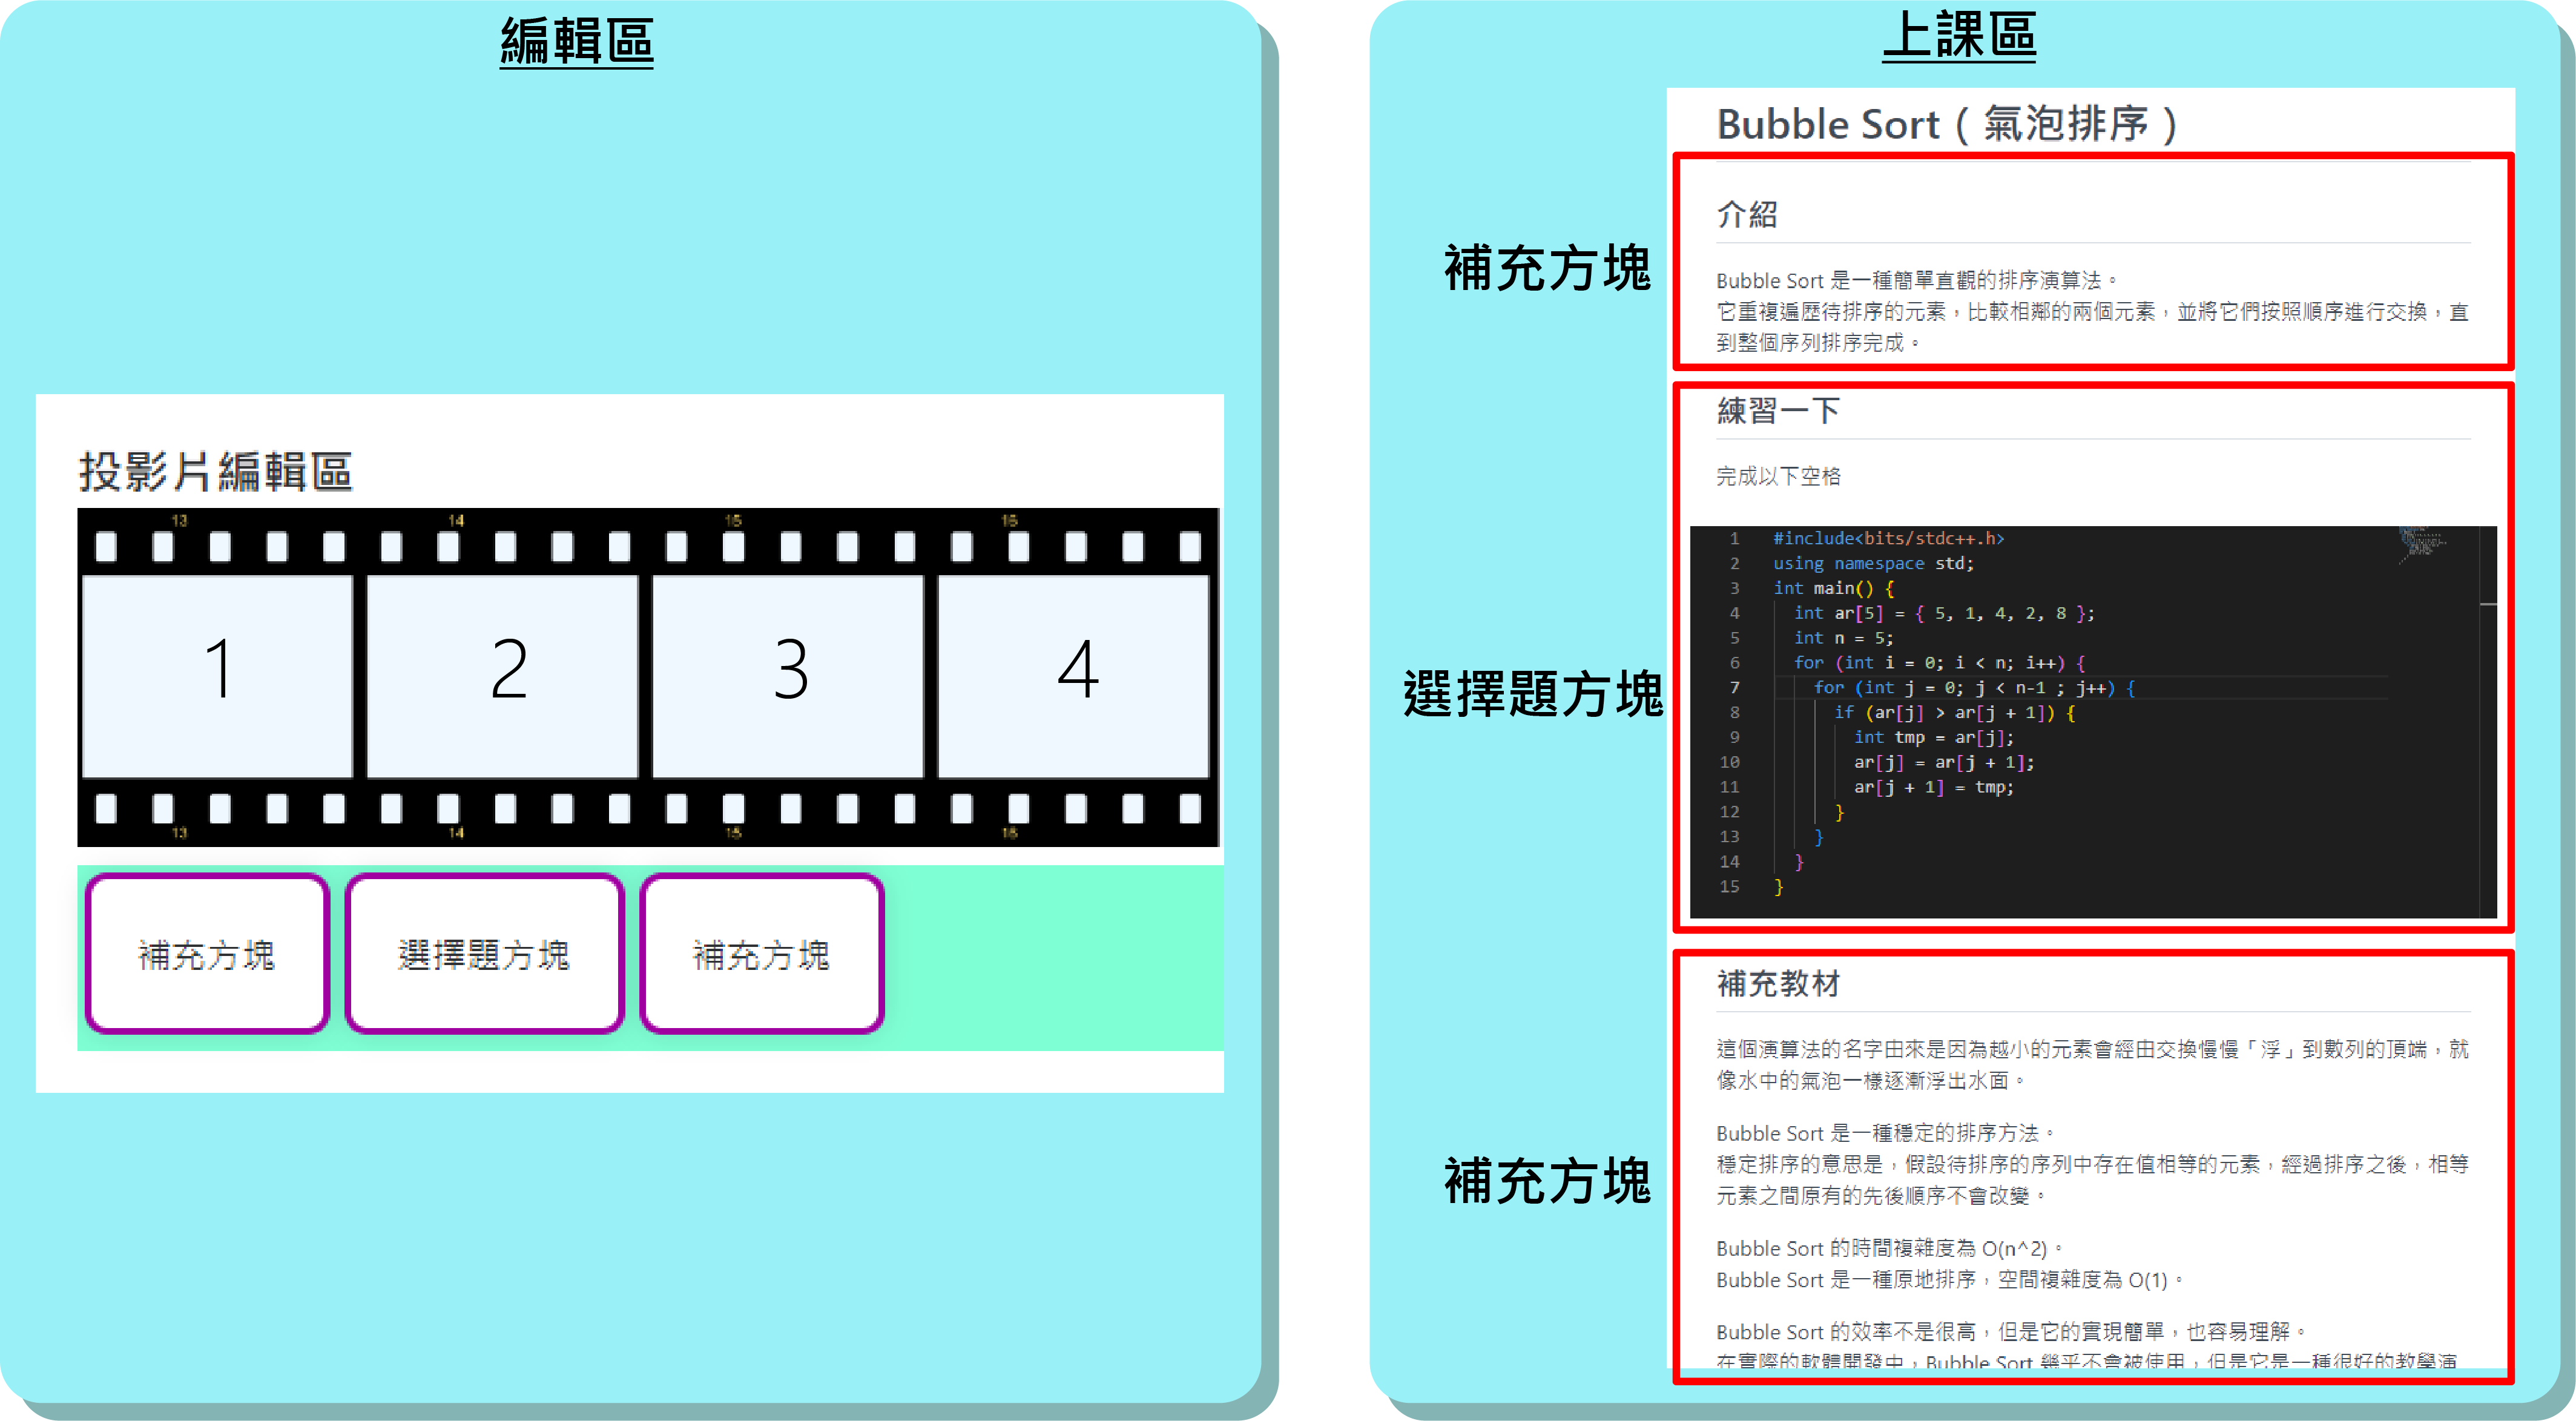
\includegraphics[width=1\textwidth]{images/timezone.png}
      %   }
      \caption{講義編輯邏輯}
      \label{fig:time}
    \end{subfigure}
    \begin{subfigure}{0.5\linewidth}
      \centering
      %   \href{https://raw.githubusercontent.com/programingtw/proglearn-plan/main/img/course.png}{ 
      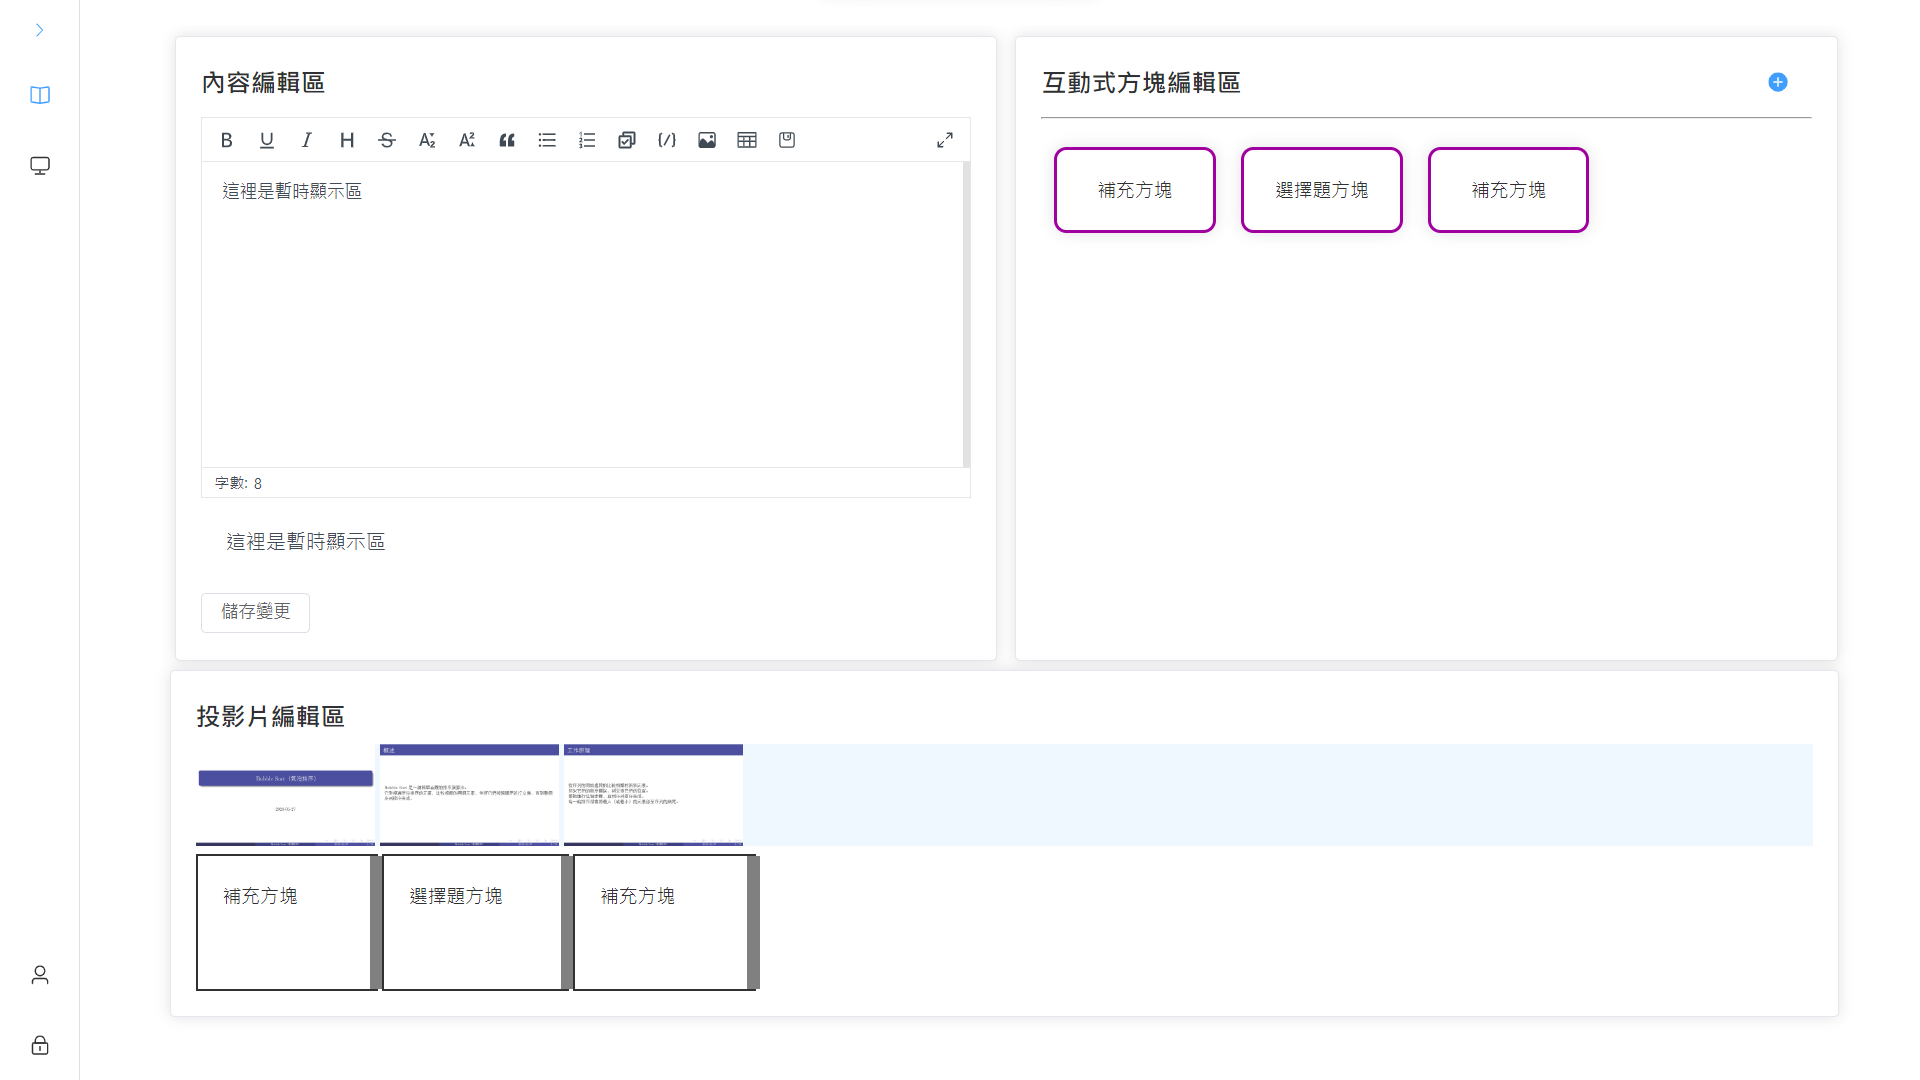
\includegraphics[width=1\textwidth]{images/edit.png}
      %   }
      \caption{講義編輯頁面}
      \label{fig:edit}
    \end{subfigure}
    \caption{講義編輯功能}
  \end{figure}

\end{enumerate}

\subsubsection{課程與作業管理}

該系統在課堂外,提供了課程與作業管理的功能(圖\ref{fig:course}、圖\ref{fig:homework})。教師可以在此設定課程章節、作業、測驗、考試與查看學生作答狀況。學生可以在此查看課程資訊、撰寫作業並得到即時批改。

\begin{figure}[H]
  \begin{subfigure}{0.5\linewidth}
    \centering
    %   \href{https://raw.githubusercontent.com/programingtw/proglearn-plan/main/img/list.png}{ 
    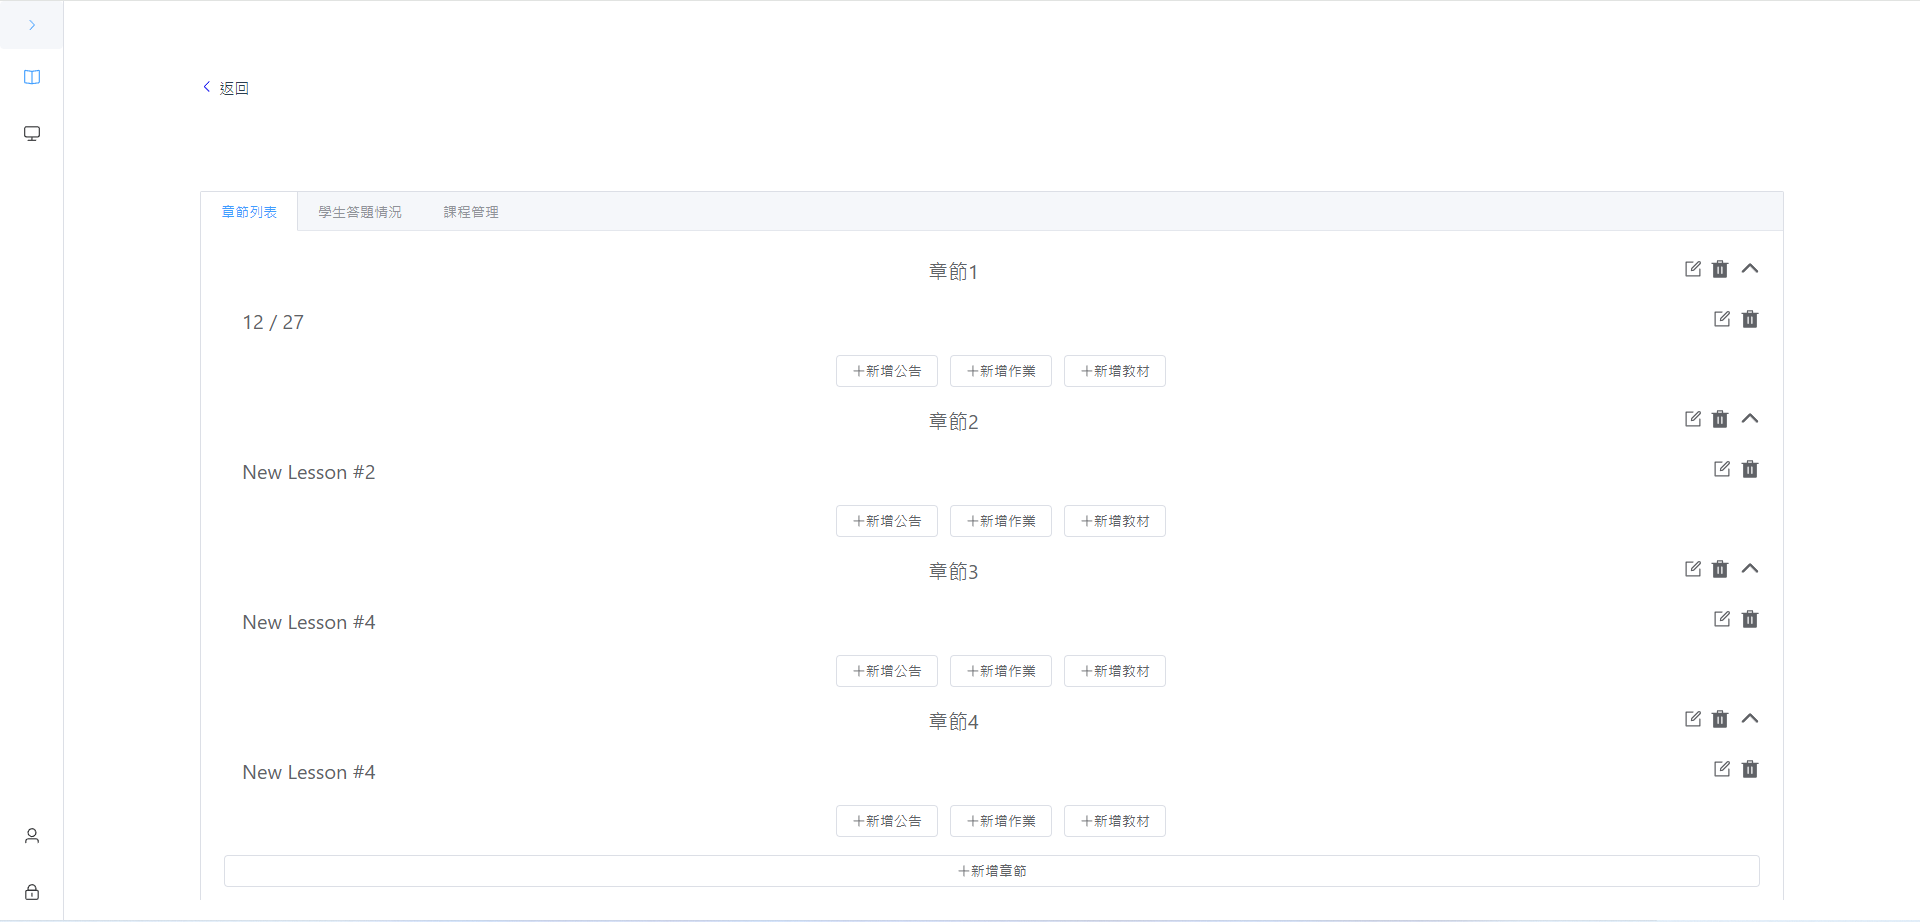
\includegraphics[width=1\textwidth]{images/chapter.png}
    %   }
    \caption{課程章節}
  \end{subfigure}
  \begin{subfigure}{0.5\linewidth}
    \centering
    %   \href{https://raw.githubusercontent.com/programingtw/proglearn-plan/main/img/course.png}{ 
    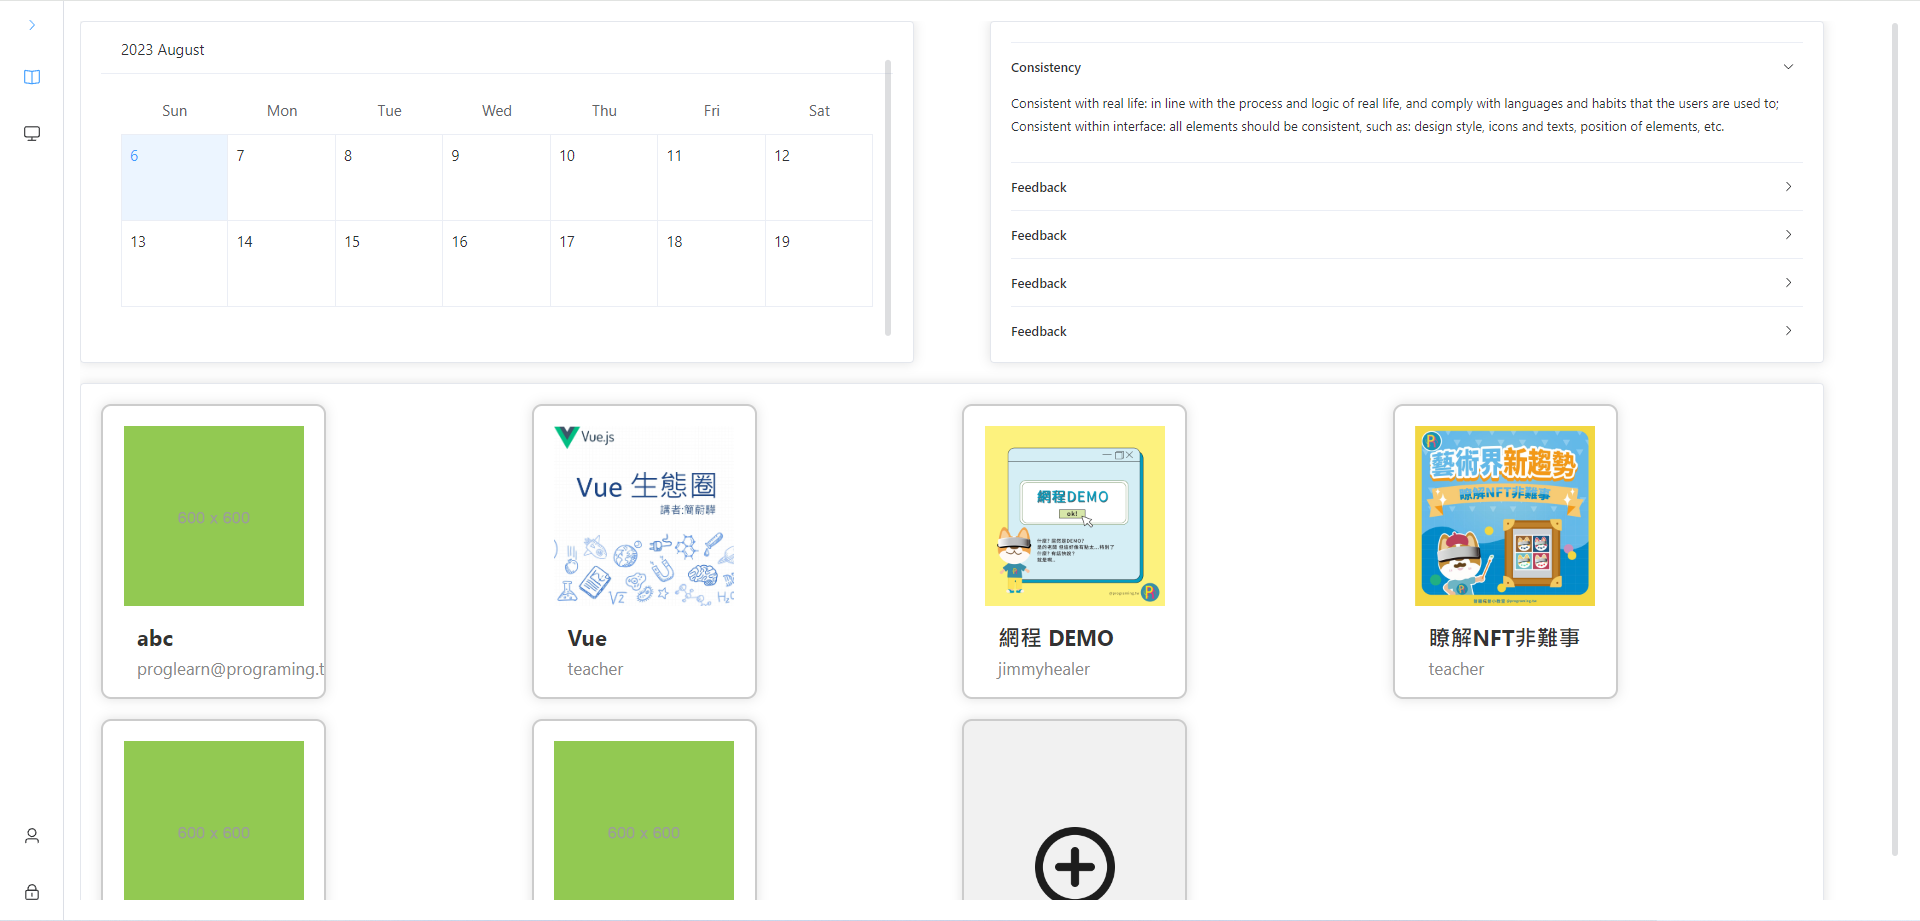
\includegraphics[width=1\textwidth]{images/course.png}
    %   }
    \caption{課程清單}
  \end{subfigure}
  \caption{課程相關頁面}
  \label{fig:course}
\end{figure}

\begin{figure}[H]
  \begin{subfigure}{0.5\linewidth}
    \centering
    %   \href{https://raw.githubusercontent.com/programingtw/proglearn-plan/main/img/list.png}{ 
    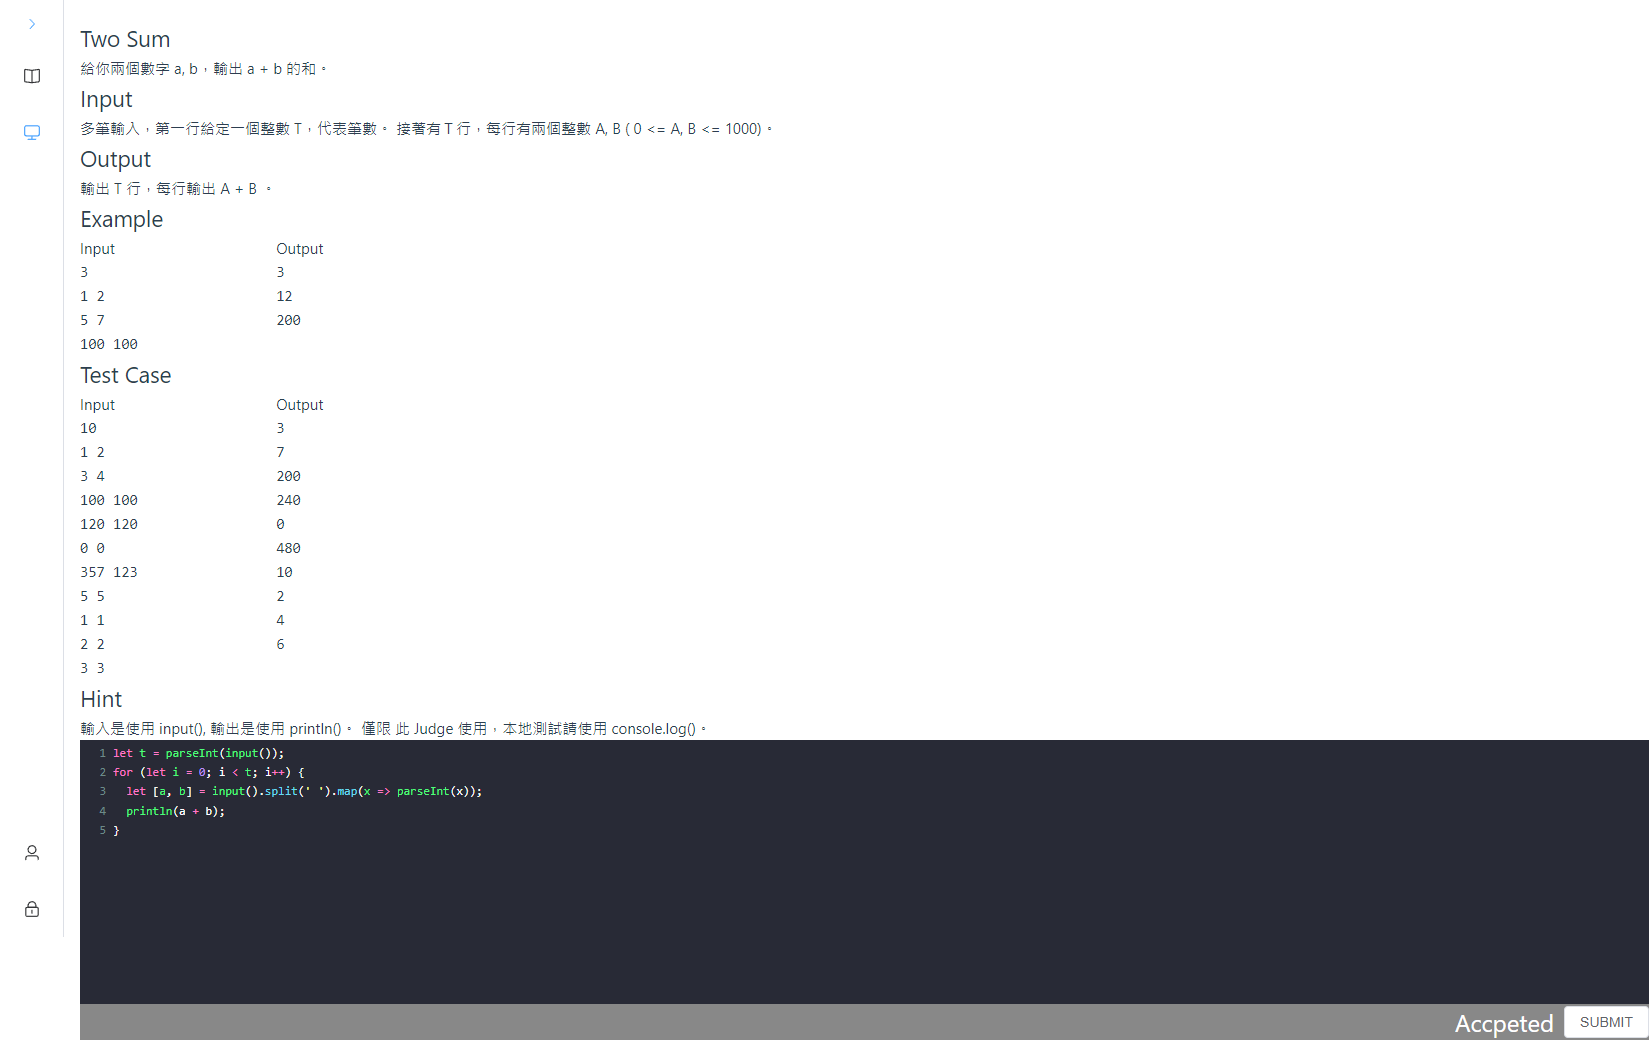
\includegraphics[width=1\textwidth]{images/homework.png}
    %   }
    \caption{作業作答}
  \end{subfigure}
  \begin{subfigure}{0.5\linewidth}
    \centering
    %   \href{https://raw.githubusercontent.com/programingtw/proglearn-plan/main/img/course.png}{ 
    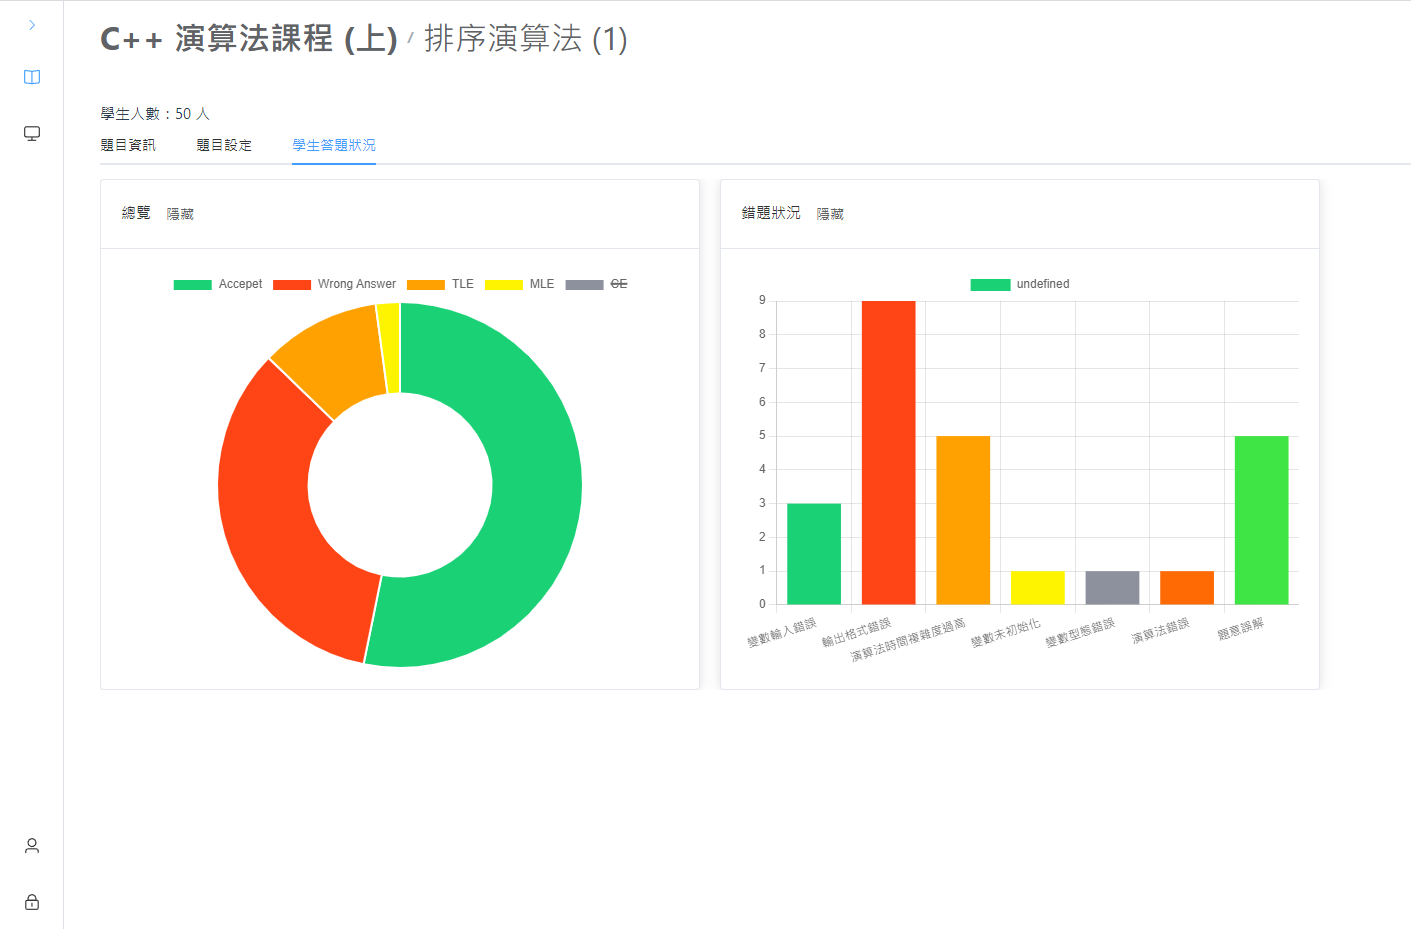
\includegraphics[width=1\textwidth]{images/feedback.png}
    %   }
    \caption{作業反饋}
  \end{subfigure}
  \caption{作業相關頁面}
  \label{fig:homework}
\end{figure}


\subsection{產品競爭優勢}

經過與大學與高中程式教師的實地訪談,我們整理出以下三個時間段的教學流程:

\begin{enumerate}
  \setlength{\parindent}{2em}
  \item 課前:準備教材
    \par 在教學前,教師會準備課堂所需的講義與投影片。市場上的講義編輯功能通常是基於文件編輯器或投影片的形式,例如 Microsoft Word 、Power Point。然而這些工具的功能較為單一,沒辦法嵌入程式執行區、互動習題等與教學相關的功能。我們的系統提供滾動式講義,搭配程式執行、引導、互動習題等功能,使講義內容與課堂做連結。並使用教師講義編輯頁面,使講義更為直觀、易於操作和修改。
  \item 課中:互動教學
  \begin{itemize}
    \setlength{\parindent}{2em}
    \item 直播功能
      \par 實現直播教學的方式,能大致分為硬體與軟體,硬體上常見的有廣播與管理系統,能夠強制控制學生的畫面。軟體上則有 Zoom、Google Meet 等以視訊為主的會議平台或專為學校開發的遠端控制系統,透過網路分享教師的語音與畫面。這些工具分別有幾項問題:前者是強制控制學生電腦,無法讓學生在課堂中與老師同步實作,也無法用電腦查詢資料、觀看講義等。後者是直播的影音可能有延遲,會導致老師的教學與控制不流暢。我們的特色是讓學生能夠在課堂中,操控投影片回顧上課內容,還能同時觀看補充講義、實作程式碼、回答習題等,讓學生就算在課堂中也能回顧與實作,並以更低延遲的直播投影片取代影像直播,使學習更為流暢。
    \item 引導功能
      \par 如何讓學生在課堂中更有參與感並且理解教學內容。市場上的一般教學軟體或平台通常缺乏對於學生學習的引導功能。我們的平台嘗試解決這個問題,透過互動區的黃色框線,在講義中顯示對應的位置,讓學生能夠清楚知道老師目前講解的內容與講義之間的對應。這樣的引導功能可以讓學生更容易理解並隨著教學進度進行,同時也能在回顧時更加方便。
  \end{itemize}
  \item 課後:課程回顧
  \par 在市場上,許多教學平台提供課後回放功能,讓學生能夠在課程結束後回顧老師的教學內容。我們的平台也提供了這樣的功能,讓學生能夠在課後拖動時間軸,回放過去的上課直播,以便進一步學習和復習。不過,我們的特色在於,課後回放不僅僅限於觀看直播畫面,還能夠觀看補充講義、實作程式碼等,並搭配引導功能,讓學生在回顧時更為全面與深入。\\
\end{enumerate}

\par 綜合以上幾點,我們整理了老師上課時可能會用到的工具並做比較:
\begin{table}[htbp]      
  \centering
  \begin{tabular}{|c|c|c|c|c|c|}
    \hline
    \thead{功能} & \thead{本系統} & \thead{Google Meet} & \thead{遠端控制系統} & \thead{CodingBar}  & \thead{廣播與管理系統}\\ 
    \hline
    直播延遲 & 低 & 高 & 高 & 高 & 低 \\ 
    \hline
    教學方式 & 線上與實體皆可 & 線上 & 實體 & 線上 & 實體 \\ 
    \hline
    電腦控制 &  &  & 遠端控制 &  & 完全控制 \\ 
    \hline
    課後回顧 & \checkmark &  &  & \checkmark &  \\ 
    \hline
    線上練習 & \checkmark &  &  & \checkmark &\\ 
    \hline
    教學功能整合 & \checkmark &  &  & \checkmark &\\ 
    \hline
  \end{tabular}
  \caption{上課工具比較表}
\end{table}
本系統在直播延遲、教學方式、課後回顧、線上練習以及教學功能整合方面表現出色,並減少對學生電腦的控制,提供了較佳的教學彈性和互動。

\newpage
\subsection{商業模式}

\subsubsection{獲利模式} % 收益流

針對不同用戶有不同的收費模式,分為B2B\footnote{B2B:Business to Business,指企業對企業的商業模式。}(學校端)與B2C\footnote{B2C:Business to Consumer,指企業對消費者的商業模式。}(教師端)兩種收費模式:

\begin{enumerate}
  \setlength{\parindent}{2em}
  \item B2B(學校端)
  \par 針對學校、補教業者、企業等機構提供專案設計與教學系統建置的服務。協助機構架設教學系統於自家伺服器上,並提供技術支援。收費模式為一次性專案設計費用與年度授權費用,其專案設計費用依據機構規模與使用人數而定,年度授權費用應收取所有教師及其課程10\%的收益。
  \item B2C(教師端)
  \par 針對個體教師提供教學系統的服務。在我們建置的線上教學系統上,提供教師月訂閱制的付費帳號,並提供技術支援。收費模式為月訂閱制費用,其費用是抽取該教師所有課程5\%的收益。
\end{enumerate}

\subsubsection{合作模式} % 關鍵合作夥伴

針對不同的合作夥伴有不同的合作模式:

\begin{enumerate}
  \setlength{\parindent}{2em}
  
  \item 國高中學校
  \par 每年教育部舉辦兩次校園數位內容與教學軟體的公開徵求活動,我們將以此為目標瞭解學校的需求,並提供必要的技術支援和服務。
  \par 在基層教育環境中驗證產品的可行性,並根據使用者的反饋進行調整。目前,我們已與臺中市立東山高級中學的資訊科技教師建立了良好的合作關係,深入了解國中和高中教師在教學上遇到的問題和需求。並針對ProgLearn進行了初步測試與改進。
  \par 我們將與機構進行試點合作,在實際教學中應用ProgLearn,對其進行教學效果的驗證。當其具備良好的教學效果後,將以此作為我們的合作案例,進一步推廣至其他學校。
  \item 補教業者
  \par 新課綱納程式設計,程式設計補教業的詢問量約增加3成\cite{ref:補教業者}。並且在智慧學習業者銷售客戶類型的占比中,資訊補習班佔補教機構的比例大幅提升,從民國110年的1.3\%提升至111年的10\%\cite{ref:110產業產值調查報告}\cite{ref:111產業產值調查報告}。顯示其市場需求的增加。
  \par 大型補教業者如三貝德、卓越、學習王科技等,皆積極拓展B2B業務。透過ProgLearn針對互動式教學、即時反饋的特色,可針對補習班的需求進行部分功能的系統整合與模組設計,提供技術支援與服務。
  \par 此外,線上教學具有較高的彈性,對於實體補習班以及大型補教業者,能夠減少教室空間的限制以及教師的通勤成本,並提供更高的教學人數上限。這對於補教業者而言,能夠提高教學效率,並且降低成本。
  \item 個體教師
  \par 2019年的新聞表示,新學期開始有高達54.4\%的學生有擔任家教的規劃\cite{ref:家教}。並且在家教市場中,程式設計的時薪可以高達2000元以上\cite{ref:學生數量},對於大學生而言,是一個不錯的兼職選擇。此外,截自2024年2月16日為止,AmazingTalker線上家教平台有9028名程式家教\footnote{https://tw.amazingtalker.com/tutor-price/programming}、1111家教網有2476筆程式教學履歷\footnote{https://tutor.1111.com.tw/}、PRO360達人網有2003名程式家教\footnote{https://www.pro360.com.tw/category/programming\_course},具有相當可觀的教師數量。
  \par 透過ProgLearn,能為個體教師提供完整的教學系統,也降低了成為教師所需的技術門檻與教學的準備成本。並且比起傳統的家教方式,線上教學具有更高的彈性,能減少通勤成本與教學空間的限制。而如果是在Hahow好學校\footnote{https://hahow.in/}、HiSKIO等線上教學平台上教學\footnote{https://hiskio.com/},不但具有較高的開課與教學門檻,平台上販售的課程還需抽取50\%的分潤,對於教師都是高昂的成本與負擔。
\end{enumerate}
